\section{ITK OpenCV Bridge}


\centeredlargetext{white}{black}{
ITK OpenCV Bridge
}

\begin{frame}
\frametitle{Introduction}
\begin{itemize}
\item ITK Module for working with other libraries
\item Moving frame and/or video data between OpenCV and ITK
\item Bring biomedical and computer vision folks together
\item \url{https://github.com/itkvideo/ITK}
\end{itemize}
\end{frame}

\begin{frame}
\frametitle{Funding Source}
\begin{itemize}
\item Contract from the National Library of Medicine (HHSN276201000579P)
\item Algorithms, Adapters \& Data Distribution Outreach 2010:
  Increasing the Impact of the Insight Toolkit (ITK)
\end{itemize}
\end{frame}

\begin{frame}
\frametitle{Design Choices}
\begin{itemize}
\item OpenCV users and ITK users should both be comfortable
\item Image to image utility functions
\item cv::Source to itk::VideoStream
\item (Later) Focus on performance
\end{itemize}
\end{frame}

\centeredlargetext{white}{black}{
Basic Image Filtering (Revisited)
}

\begin{frame}
\frametitle{Include Header Files}
\framesubtitle{ITKOpenCVBridge/exercise1/Ex1\_BasicFilteringOpenCVBridge.cxx}
\begin{itemize}
\item We include ITK and OpenCV headers (like before):
\lstlistingwithnumber{20}{21}{Ex1_BasicFilteringOpenCVBridge.cxx}
\lstlistingwithnumber{23}{24}{Ex1_BasicFilteringOpenCVBridge.cxx}
\item We also need to include the bridge header:
\lstlistingwithnumber{25}{25}{Ex1_BasicFilteringOpenCVBridge.cxx}
\end{itemize}
\end{frame}

\begin{frame}
\frametitle{Basic Layout}
\framesubtitle{ITKOpenCVBridge/exercise1/Ex1\_BasicFilteringOpenCVBridge.cxx}
\begin{itemize}
\item The basic layout of this file is the same as the OpenCV
  Examples:
\lstlistingwithnumber{27}{35}{Ex1_BasicFilteringOpenCVBridge.cxx}
\lstlistingwithnumber{69}{84}{Ex1_BasicFilteringOpenCVBridge.cxx}
\end{itemize}
\end{frame}

\begin{frame}
\frametitle{Adding ITK}
\framesubtitle{ITKOpenCVBridge/exercise1/Ex1\_BasicFilteringOpenCVBridge.cxx}
\begin{itemize}
\item The type definitions should also be familiar from the ITK
  Material:
\lstlistingwithnumber{38}{45}{Ex1_BasicFilteringOpenCVBridge.cxx}
\item However, notice the bridge class. It contains the conversion function
between OpenCV and ITK.
\lstlistingwithnumber{42}{42}{Ex1_BasicFilteringOpenCVBridge.cxx}
\end{itemize}
\end{frame}

\begin{frame}
\frametitle{From OpenCV to ITK}
\framesubtitle{ITKOpenCVBridge/exercise1/Ex1\_BasicFilteringOpenCVBridge.cxx}
\begin{itemize}
\item We call our conversion function to go from a cv::Mat to an
  itk::Image
\lstlistingwithnumber{47}{48}{Ex1_BasicFilteringOpenCVBridge.cxx}
\end{itemize}
\end{frame}

\begin{frame}
\frametitle{Filtering with ITK}
\framesubtitle{ITKOpenCVBridge/exercise1/Ex1\_BasicFilteringOpenCVBridge.cxx}
\begin{itemize}
\item The median filtering is normal ITK code, but we do not connect our
output to a writer
\lstlistingwithnumber{49}{64}{Ex1_BasicFilteringOpenCVBridge.cxx}
\pause
\item Instead, we set it to our conversion function
\lstlistingwithnumber{66}{67}{Ex1_BasicFilteringOpenCVBridge.cxx}
\end{itemize}
\end{frame}

\begin{frame}
\frametitle{Running the Example}
\framesubtitle{ITKOpenCVBridge/exercise1/Ex1\_BasicFilteringOpenCVBridge.cxx}
\begin{itemize}
\item Running the example the same way as before, we see a nicely
median-filtered image.
\pause
\item Now, the fun part. Let's modify our example to use Curvature Flow, an
anisotropic diffusion filter built into ITK.
\end{itemize}
\end{frame}

\begin{frame}
\begin{itemize}
\frametitle{Exercise 1}
\framesubtitle{ITKOpenCVBridge/exercise1/Ex1\_BasicFilteringOpenCVBridge.cxx}
\item Hint 1: Curvature Flow requires {\tt float} as the output pixel
  type.
\pause
\item Hint 2: Curvature Flow does not take a radius parameter. It's
  salient functions are:
\lstlistingwithnumber{50}{51}{Ex1_BasicFilteringOpenCVBridgeAnswer.cxx}
\end{itemize}
\end{frame}

\begin{frame}
\begin{itemize}
\frametitle{Exercise 1: Answer}
\framesubtitle{ITKOpenCVBridge/exercise1/Ex1\_BasicFilteringOpenCVBridgeAnswer.cxx}
\item First, change the included filter
\lstlistingwithnumber{24}{24}{Ex1_BasicFilteringOpenCVBridgeAnswer.cxx}
\pause
\item The type definitions also need to change to reflect the new
  filter and output image types.
\lstlistingwithnumber{37}{44}{Ex1_BasicFilteringOpenCVBridgeAnswer.cxx}
\end{itemize}
\end{frame}

\begin{frame}
\begin{itemize}
\frametitle{Exercise 1: Answer}
\framesubtitle{ITKOpenCVBridge/exercise1/Ex1\_BasicFilteringOpenCVBridgeAnswer.cxx}
\item The semantics of calling the filter also has to change:
\lstlistingwithnumber{50}{51}{Ex1_BasicFilteringOpenCVBridgeAnswer.cxx}
\pause
\item That's it! Now you're using a ``better'' blurring scheme.
\end{itemize}
\end{frame}

\begin{frame}
\begin{itemize}
\frametitle{Exercise 1: Answer}
\framesubtitle{ITKOpenCVBridge/exercise1/Ex1\_BasicFilteringOpenCVBridgeAnswer.cxx}
\item The final pipeline should look like this:
\lstlistingwithnumber{35}{35}{Ex1_BasicFilteringOpenCVBridgeAnswer.cxx}
\lstlistingwithnumber{46}{62}{Ex1_BasicFilteringOpenCVBridgeAnswer.cxx}
\end{itemize}
\end{frame}

\begin{frame}
\begin{itemize}
\frametitle{Exercise 1: Answer}
\framesubtitle{ITKOpenCVBridge/exercise1/Ex1\_BasicFilteringOpenCVBridgeAnswer.cxx}
\item The results should look like this:
\end{itemize}
\begin{columns}[c]
\column{0.33\textwidth}
\begin{center}
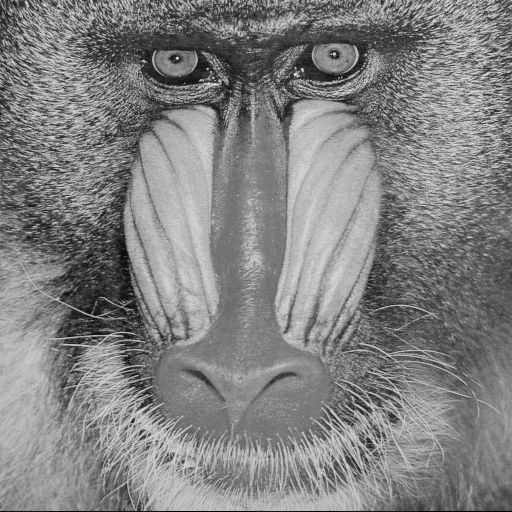
\includegraphics[width=1\textwidth]{mandrilgray.png} \\
Original
\end{center}
\column{0.33\textwidth}
\begin{center}
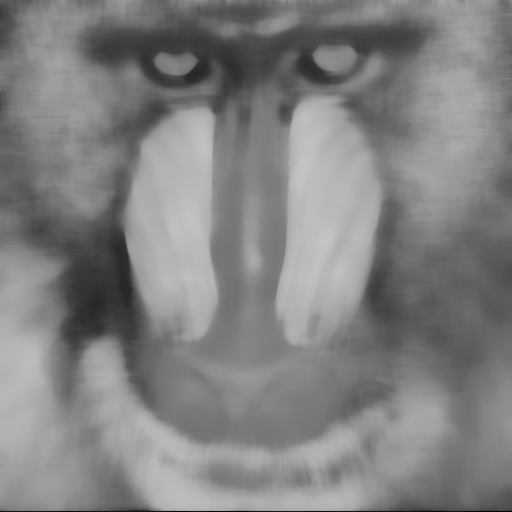
\includegraphics[width=1\textwidth]{OpenCVITKex1.png} \\
Median Filter
\end{center}
\column{0.33\textwidth}
\begin{center}
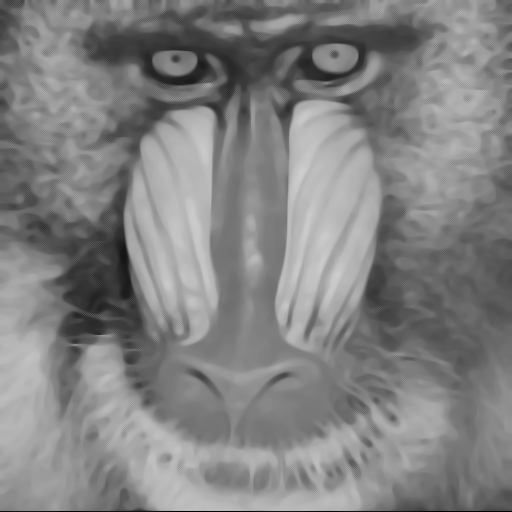
\includegraphics[width=1\textwidth]{OpenCVITKex1-ans.png} \\
Curvature Flow
\end{center}
\end{columns}
\end{frame}

\centeredlargetext{white}{black}{
Basic Video Filtering (Revisited)
}

\begin{frame}
\frametitle{Basic Layout}
\framesubtitle{ITKOpenCVBridge/exercise2/Ex2\_BasicFilteringOpenCVBridge.cxx}
\begin{itemize}
\item The basic layout of this file is the same as the OpenCV Video
  Examples:
\item There are three functions as before.
\lstlistingwithnumber{28}{28}{Ex2_BasicFilteringOpenCVBridge.cxx}
\lstlistingwithnumber{63}{63}{Ex2_BasicFilteringOpenCVBridge.cxx}
\lstlistingwithnumber{89}{89}{Ex2_BasicFilteringOpenCVBridge.cxx}
\pause
\item We only need to modify {\tt processFrame} to incorporate ITK.
\end{itemize}
\end{frame}

\begin{frame}
\frametitle{Filtering with ITK}
\framesubtitle{ITKOpenCVBridge/exercise2/Ex2\_BasicFilteringOpenCVBridge.cxx}
\begin{itemize}
\item The median filtering is again normal ITK code.
\lstlistingwithnumber{28}{29}{Ex2_BasicFilteringOpenCVBridge.cxx}
\lstlistingwithnumber{39}{60}{Ex2_BasicFilteringOpenCVBridge.cxx}
\end{itemize}
\end{frame}

\begin{frame}
\begin{itemize}
\frametitle{Exercise 2}
\framesubtitle{ITKOpenCVBridge/exercise2/Ex2\_BasicFilteringOpenCVBridge.cxx}
\item Let's modify this example to use the same canny edge detection
  from the ITK examples
\pause 
\item Hint 1: You should use the following function instead of ITK's
cast image filter for producing output
\lstlistingwithnumber{72}{72}{Ex2_BasicFilteringOpenCVBridgeAnswer.cxx}
\pause
\item Hint 2: You should only have to modify {\tt processFrame}
\end{itemize}
\end{frame}

\begin{frame}
\begin{itemize}
\frametitle{Exercise 2: Answer}
\framesubtitle{ITKOpenCVBridge/exercise2/Ex2\_BasicFilteringOpenCVBridgeAnswer.cxx}
\item You should now have some extra typedefs:
\lstlistingwithnumber{39}{44}{Ex2_BasicFilteringOpenCVBridgeAnswer.cxx}
\end{itemize}
\end{frame}

\begin{frame}
\begin{itemize}
\frametitle{Exercise 2: Answer}
\framesubtitle{ITKOpenCVBridge/exercise2/Ex2\_BasicFilteringOpenCVBridgeAnswer.cxx}
\item Your new ITK pipeline will look like this:
\lstlistingwithnumber{46}{67}{Ex2_BasicFilteringOpenCVBridgeAnswer.cxx}
\end{itemize}
\end{frame}

\begin{frame}
\begin{itemize}
\frametitle{Exercise 2: Answer}
\framesubtitle{ITKOpenCVBridge/exercise2/Ex2\_BasicFilteringOpenCVBridgeAnswer.cxx}
\item Your new ITK pipeline will look like this:
\lstlistingwithnumber{69}{74}{Ex2_BasicFilteringOpenCVBridgeAnswer.cxx}
\end{itemize}
\end{frame}